\section{E-commerce Overview}
\label{sec:e_commerce_overview}
“Interaction between communication systems, data management systems and security, which because of them exchange commercial information in relation to the sale products or services, will be available, so the definition, the main components of electronic commerce are: communication systems, data management systems and security \cite{commerce_intro_1}.”
\newline
Today, most of the population, use these virtual stores to shop or simply to inquire. In fact, these systems allow for a timely basis to have information regarding the good we are seeking. In this way these systems help the customer in buying a particular good.
\newline
\begin{figure}[htb]
 \centering
 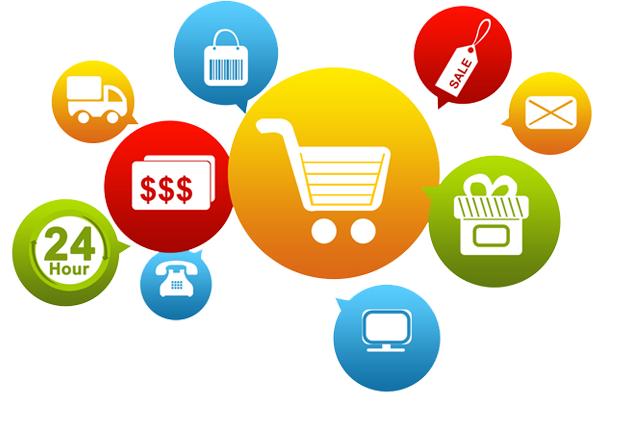
\includegraphics[width=0.8\linewidth]{images/chapter1/e-commerce.png}\hfill
 \caption[e-commerce overview]{e-commerce overview}
 \label{fig:e_commerce_overview}
\end{figure}
The e-commerce in Europe has continued to grow even if at different rates and in different ways in different countries. Online shopping is a habit well established in Britain, Germany and France, markets that together account for 70-80\% of e-commerce Europe, while it is just starting out or is growing in the rest of Europe, including countries such as Italy and Spain. The most rapid growth, however, affect the emerging economies of Eastern Europe, led by Russia, the market for which is expected to grow by up to 200\% over the next three years.
\newline
In mature markets, growth was driven primarily by an increase in the frequency of purchase by the consumer and by the tendency to spend more through online channels, while in countries where e-commerce is developing growth results especially by the increase in online shoppers \cite{e_commerce_in_italy}.
\newline
The moobile is the key factor in the growth of e-commerce. The diffusion of smartphones and tablets has extended much access to the online market, even in Italy, where 29 million end users access the Internet from the mobile. Companies that have not addressed this change have had a decline in the conversion rate on its website, while those who understood the new opportunities brought by the new type of access has been able to develop the offer of additional products and services dedicated, for example taking advantage of the geolocation of the customer. New entrants are mainly the physical stores, which saw in e-commerce for a way to expand its customer base, and producers of goods and services, they see the distribution companies increasingly as an obstacle to profitability.
What are the advantages and disadvantages (risks) of a system of e-commerce?
\newline
\subsection{Advantages and disadvantages of a system of e-commerce}
The benefits of electronic commerce are general (system-wide) and specific for the seller or the buyer.
\begin{itemize}
  \item Benefits for system:
  \begin{itemize}
    \item It is a global phenomenon and that a potentially global market;
    \item the transactions can develop throughout the day without interruption and realtime;
    \item the interaction between the parties can be synchronous or asynchronous;
    \item there is greater operational flexibility of relations between the parties.
  \end{itemize}

  \item Benefits for buyer:
  \begin{itemize}
    \item \emph{amenity}: e-commerce stores are always open every day including holidays: just a few clicks from home or from work to buy what you want. The convenience to receive the goods directly at home is an important added value: we forget the long lines in the parking lot and in front of the chest of the crowded malls and you live a better buying experience;
    \item \emph{convenience}: a purchase through the Web is much more convenient. In addition to the discounts and promotions who flock the network there is convenience in movement (no need to move by car or public services) and in the time saved;
    \item \emph{information}: buying on the Internet allows you to calmly assess the choice of major purchases due to the large amount of information that you can easily find, to the advice and comments from other consumers, the wide range of products and alternatives;
  \end{itemize}
  \item Benefits for seller:
    \begin{itemize}
    \item the \emph{flexibility} according to your needs of its commitments is easy to plan a few hours each day to devote to a new major project sales with the Internet. The mailbox collects communications and orders will be processed as soon as possible;
    \item \emph{visibility}: there is no place in the world frequented the Internet, after an initial phase of advertising the same managers are surprised of the amount of visits and contacts received. Those who already have a business and want to open a new sales channel with the Internet, should not overlook the excellent positive return in terms of image that the site produces and that also benefits traditional activity;
    \item the \emph{economy}: starting a new project sales with Internet does not require large investments and for the creation of storefront, both for advertising, both for the organization. Furthermore a good design e-commerce based on appropriate contacts with the suppliers allows to reduce to a minimum investment of stock.
  \end{itemize}
\end{itemize}
Companies that sell products or services on the Internet to be successful must obtain credibility and visibility on the Web and to achieve this it is not enough to have a secure server. To get credibility companies need to know how to build for the users of their website, a positive experience not only during the purchasing process, but also before and after, so that the user wants to repeat the experience and advice to other users. Creating a positive experience for their customers and by advertising messages and techniques of SEO companies build a reputation or image of successful enterprise.
\newline
In face-to-face transactions, customers and sellers use a number of physical signals to determine that they are dealing with a trustworthy partner. Retailers can check signatures and identity cards of their clients; buyers can see the badges with the name of employees, try the goods carefully and retain proof of their purchases. On electronic networks, none of these methods is applicable. For this reason, have been developed (and are now fully available and effective) some control systems performing similar functions.
\newline
The low cost of entry and the ease with which text and graphics can be copied, make it possible for almost anyone to create a website that pairs represent an organization established trading. No new reports of false virtual shops look professional, created to impersonate the Web version of existing activities, in order to illegally obtain credit card numbers. This problem has been resolved. Scammers are able to intercept transmissions. A thief can work hard to get the numbers of credit cards. A competitor or a disgruntled customer can enter an error in the company's website, in order to induce him to refuse service to potential customers or initiate other unauthorized actions. Sources intentional or accidental sometimes cause changes to the content of a communication route. User's name, credit card numbers and total currency are all vulnerable to such alteration. To this we have been developed safety systems to ensure the integrity of all the phases of the transaction. The data coming from America, are explicit: the continued growth of e-commerce is comforting. A concern, however, is the security front. In fact, the problems related to information security are increasing.
\newline
You can identify two types of Internet attacks to the network:
\begin{itemize}
  \item \emph{Passive attacks}: Need to get the most information about the network in question, but does not have the purpose of hostile intrusion; (Ex. Eavesdropping: sniffing the information being sent across it in order to acquire the contents of transactions for subsequent analysis on personal data, or on behalf of third parties);
  \item \emph{Active attacks}: as a result of the information collected by passive attacks, you can attack systems identified to implement changes to the data, lock services, obtain confidential information.\ldots
\end{itemize}
Another worrying phenomenon, in terms of information security, is surely the phishing; It is an illegal system to collect sensitive data such as information about your credit card or access to bank accounts. The vast majority of messages takes place starting from phishing e-mail addresses stolen (ie where the authors have introduced illegally) or forged to perfection (in the eyes of the end user) on the basis of a known syntax or through the use of imitators sites of companies-mirror. These threats can cause a loss of integrity of databases, a loss of profits, increased costs for security systems, a critical data loss, a loss of trade secret information and damage to corporate reputation.
\newline
Systems e-commerce are the most famous Amazon, Ebay, etc..
\subsection{Amazon}
Amazon.com, Inc., often referred to as simply Amazon, is an American electronic commerce and cloud computing company with headquarters in Seattle,Washington. It is the largest Internet-based retailer in the United States.
\begin{figure}[htb]
 \centering
 
\includegraphics[width=0.4\linewidth]{images/chapter1/amazon_logo.jpg}\hfill
 \caption[Amazon logo]{Amazon logo}
 \label{fig:amazon_logo}
\end{figure}
Amazon.com started as an online bookstore, later diversifying to sell DVDs, Blu-rays, CDs, videodownloads/streaming, MP3 downloads/streaming, audiobook downloads/streaming, software, video games, electronics, apparel, furniture, food, toys and jewelry. The company also produces consumer electronics—notably, Amazon Kindle e-book readers, Fire tablets, Fire TV and Fire Phone - and is the world's largest provider of cloud infrastructure services (IaaS). Amazon also sells certain low-end products like USB cables under its in-house brand AmazonBasics.
\newline
Amazon has separate retail websites for United States, United Kingdom and Ireland, France, Canada, Germany, Italy, Spain, Netherlands, Australia, Brazil, Japan, China, India and Mexico.
\newline
Amazon also offers international shipping to certain other countries for some of its products. In 2011, it professed an intention to launch its websites in Poland and Sweden.
In 2015, Amazon surpassed Walmart as the most valuable retailer in the United States by market capitalization.
The company was founded in 1994, spurred by what Bezos called his “regret minimization framework,” which described his efforts to fend off any regrets for not participating sooner in the Internet business boom during that time.
\subsection{Ebay}
Ebay Inc. is an American multinational corporation and e-commerce company, providing consumer to consumer and business to consumer sales services via Internet.
\begin{figure}[htb]
  \centering
  
\includegraphics[width=0.4\linewidth]{images/chapter1/ebay_logo.jpeg}\hfill
  \caption[Ebay logo]{Ebay logo}
  \label{fig:ebay_logo}
\end{figure}
It is headquartered in San Jose, California. eBay was founded by Pierre Omidyar in 1995, and became a notable success story of the dot-com bubble. Today, it is a multibillion-dollar business with operations localized in over 30 countries. The company manages eBay.com, an online auction and shopping website in which people and businesses buy and sell a broad variety of goods and services worldwide. In addition to its auction-style sales, the website has since expanded to include “Buy It Now” shopping; shopping by UPC, ISBN, or other kind of SKU (via Half.com); online classified advertisements (via Kijijior eBay Classifieds); online event ticket trading (via StubHub); online money transfers (via PayPal) and other services.
\newline
The website is free to use for buyers, but sellers are charged fees for listing items and again when those items are sold. The company also makes additional money through its PayPal subsidiary which is used by sellers to collect payment for items sold.
\begin{figure}[htb]
 \centering
 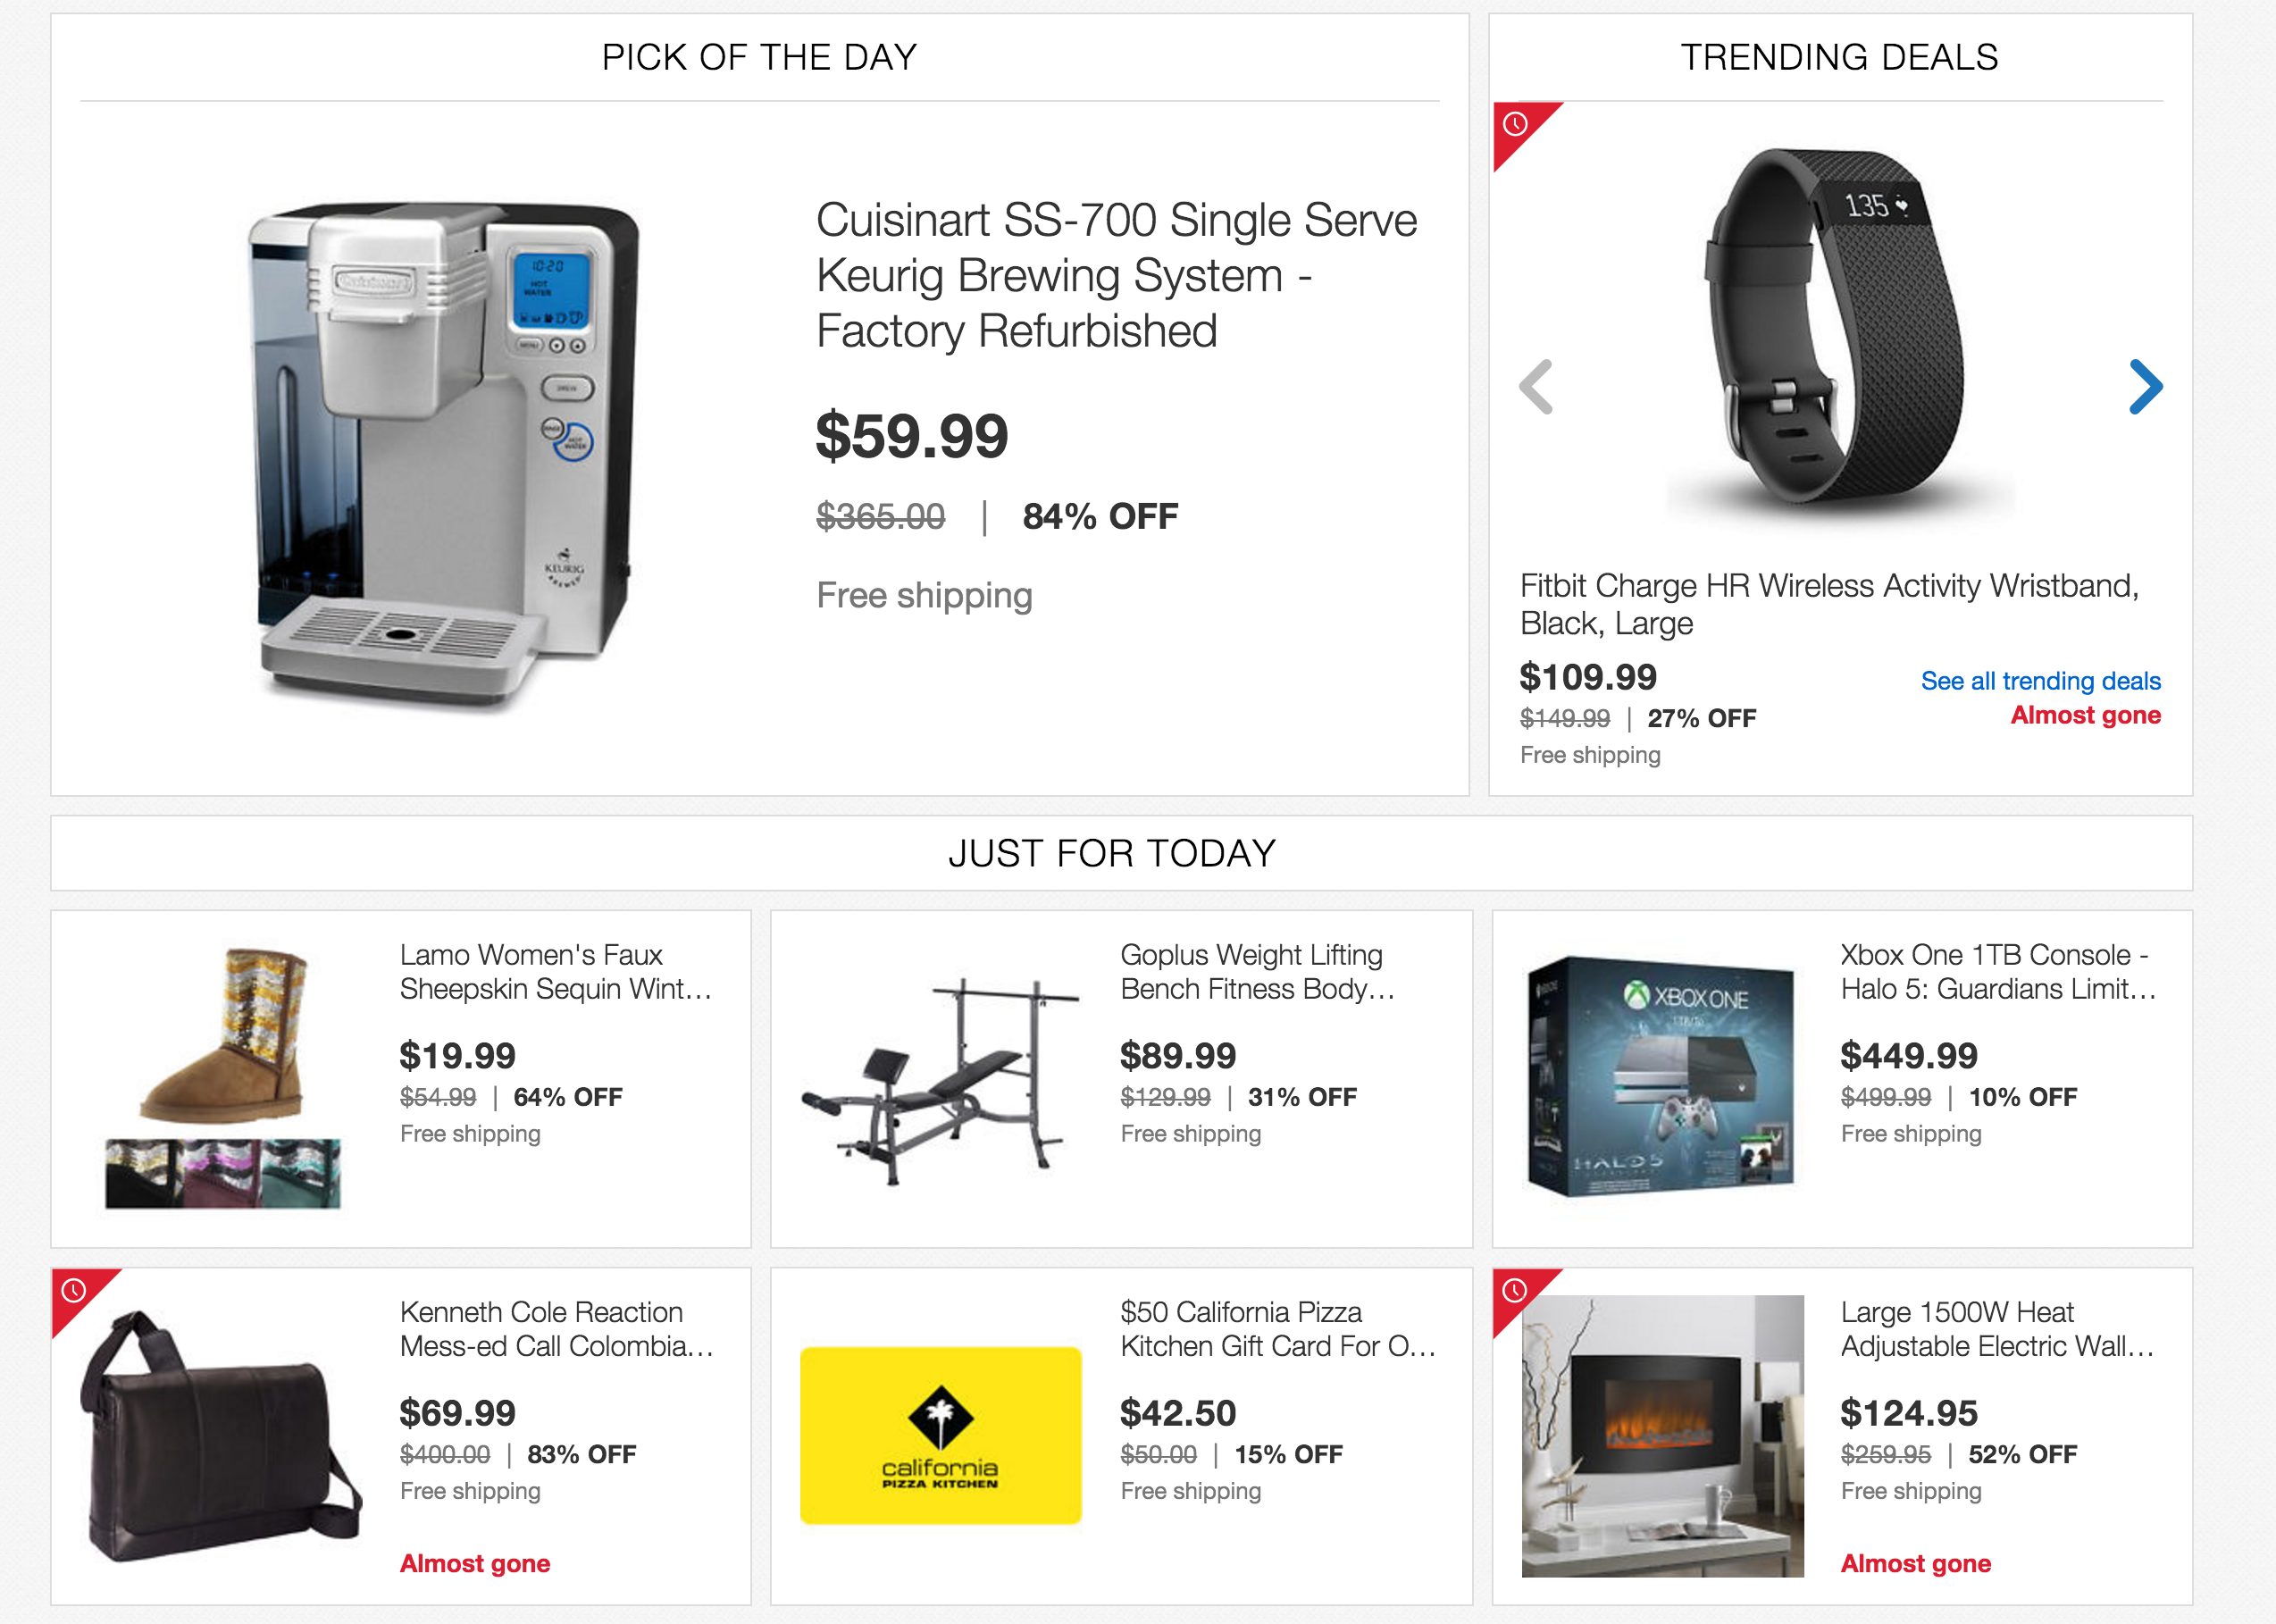
\includegraphics[width=0.9\linewidth]{images/chapter1/ex-ebay.png}\hfill
 \caption[Ebay shop]{Ebay shop}
 \label{fig:e_commerce_ebay_shop}
\end{figure}